% !TeX spellcheck = it_IT
\documentclass[a4paper,12pt]{article}

\usepackage{alltt, fancyvrb, url}
\usepackage{graphicx}
\usepackage{algorithmic}
\usepackage[utf8]{inputenc}
\usepackage{titling}
\usepackage{fancyhdr}
\usepackage{fontenc}
\usepackage{amsmath,mathtools,algorithm}
\usepackage{amssymb}
\usepackage{longtable}
\usepackage{setspace}
\usepackage{listings}
\usepackage{color}
\usepackage{eurosym}
\usepackage{array}
\usepackage[referable]{threeparttablex}
\usepackage{pifont}
\usepackage{siunitx}
\usepackage{subcaption}

\newcommand{\cmark}{\ding{51}}
\newcommand{\xmark}{\ding{55}}

\usepackage[italian,hidelinks]{hyperref}

\usepackage[italian]{babel}
\usepackage[italian]{cleveref}


\pretitle{%
	\begin{center}
		\LARGE
	}
\posttitle{\end{center}}


\title{\vspace{-5em}\Huge \textbf{Evolutionary Cars}
}
\author{
	Gabriele Graffieti \\ \small \url{gabriele.graffieti@studio.unibo.it}
	\vspace{15pt}
	\\
	Alfredo Maffi \\ \small \url{alfredo.maffi@studio.unibo.it}
	\vspace{15pt}
	\\
	Manuel Peruzzi \\ \small \url{manuel.peruzzi@studio.unibo.it}
}

\date{}

\begin{document}

\maketitle
\pagenumbering{arabic}
\tableofcontents
\newpage

\section{Introduzione}

Questo documento è la relazione del progetto Evolutionary Cars, realizzato per il corso di Sistemi Intelligenti Robotici, erogato dalla facoltà di Ingegneria e Scienze Informatiche dell'Università di Bologna (A.A. 2017/2018). Lo scopo del progetto è quello di realizzare una simulazione nella quale delle auto (2D) imparino a guidare lungo un circuito, evitandone i muri, attraverso la metodologia \emph{evolutionary robotics}. Più nel dettaglio, l'obiettivo è quello di pilotare ogni auto attraverso una rete neurale separata, ed evolvere i pesi della stessa attraverso un algoritmo genetico, di generazione in generazione.

\section{Stato dell'arte} \label{stato-dell-arte}

\section{Architettura} \label{architecture}
In questa sezione verrà illustrata l'architettura generale del sistema. La progettazione è stata effettuata in modo da isolare gli aspetti chiave da quelli relativi all'ambiente di esecuzione. Di conseguenza, il sistema risulta suddiviso in due sottoparti principali: \emph{core} e ambiente di esecuziuito. D'altro canto, la parte relativa all'ambiente di esecuzione si rivela necessaria per permettere al sistema di adattarsi ed essere eseguito in un certo ambiente, sia esso reale o virtuale. Segue una breve descrizione dei componenti del sistema.
\begin{description}
	\item[Driver Agent]: entità preposta alla guida di un'auto. Indipendentemente dall'implementazione e dalla natura del veicolo, determina la potenza del motore e la direzione di sterzata dello stesso, a partire dalle informazioni relative alla distanza dai muri del tracciato. Ogni decisione che incide sul movimento dell'auto è determinata da una rete neurale interna, i cui pesi sono regolati in modo da aderire al genotipo dell'agente.
	\item[Neural Network]: rete neurale feedforward utilizzata per pilotare un'auto. Riceve in input cinque valori di prossimità, che descrivono lo stato dell'auto in relazione ai muri del tracciato, e produce in output forza motore e direzione dello spostamento successivo. I pesi della rete sono inizialmente definiti in modo casuale, per poi essere adattati in corso d'opera in seguito all'evoluzione del genotipo corrispondente.
	\item[Genotype]: insieme di informazioni che contraddistinguono il comportamento di un'auto da un'altro. In particolare, contiene i pesi da assegnare alla \emph{neural network} di un particolare agente.
	\item[Genetic Algorithm]: algoritmo finalizzato all'evoluzione dei genotipi da una generazione alla successiva. Si compone delle fasi di selezione, crossover e mutazione, che saranno discusse nel dettaglio in \autoref{evolution}.
	\item[Controller]: può essere definito come il collante tra le parti di core e simulazione del sistema. Si occupa inizialmente di istanziare l'algoritmo genetico ed un insieme di driver agent. È responsabile dell'avvio del processo di \emph{evaluation} dei genotipi, interagendo con un componente relativo alla gestione della parte di simulazione. Al termine di tale processo viene notificato, in modo da poter poi provvedere all'avvio della fase di evoluzione, interagendo con l'algoritmo genetico.
\end{description}
In \autoref{architecture-diagram} è illustrato un diagramma che descrive, in maniera informale, l'architettura del sistema. Per quanto riguarda la parte relativa all'ambiente di esecuzione, in \autoref{simulation} verrà proposta un'infrastruttura per effettuare una simulazione del sistema.

\begin{figure}[H]
	\centering
	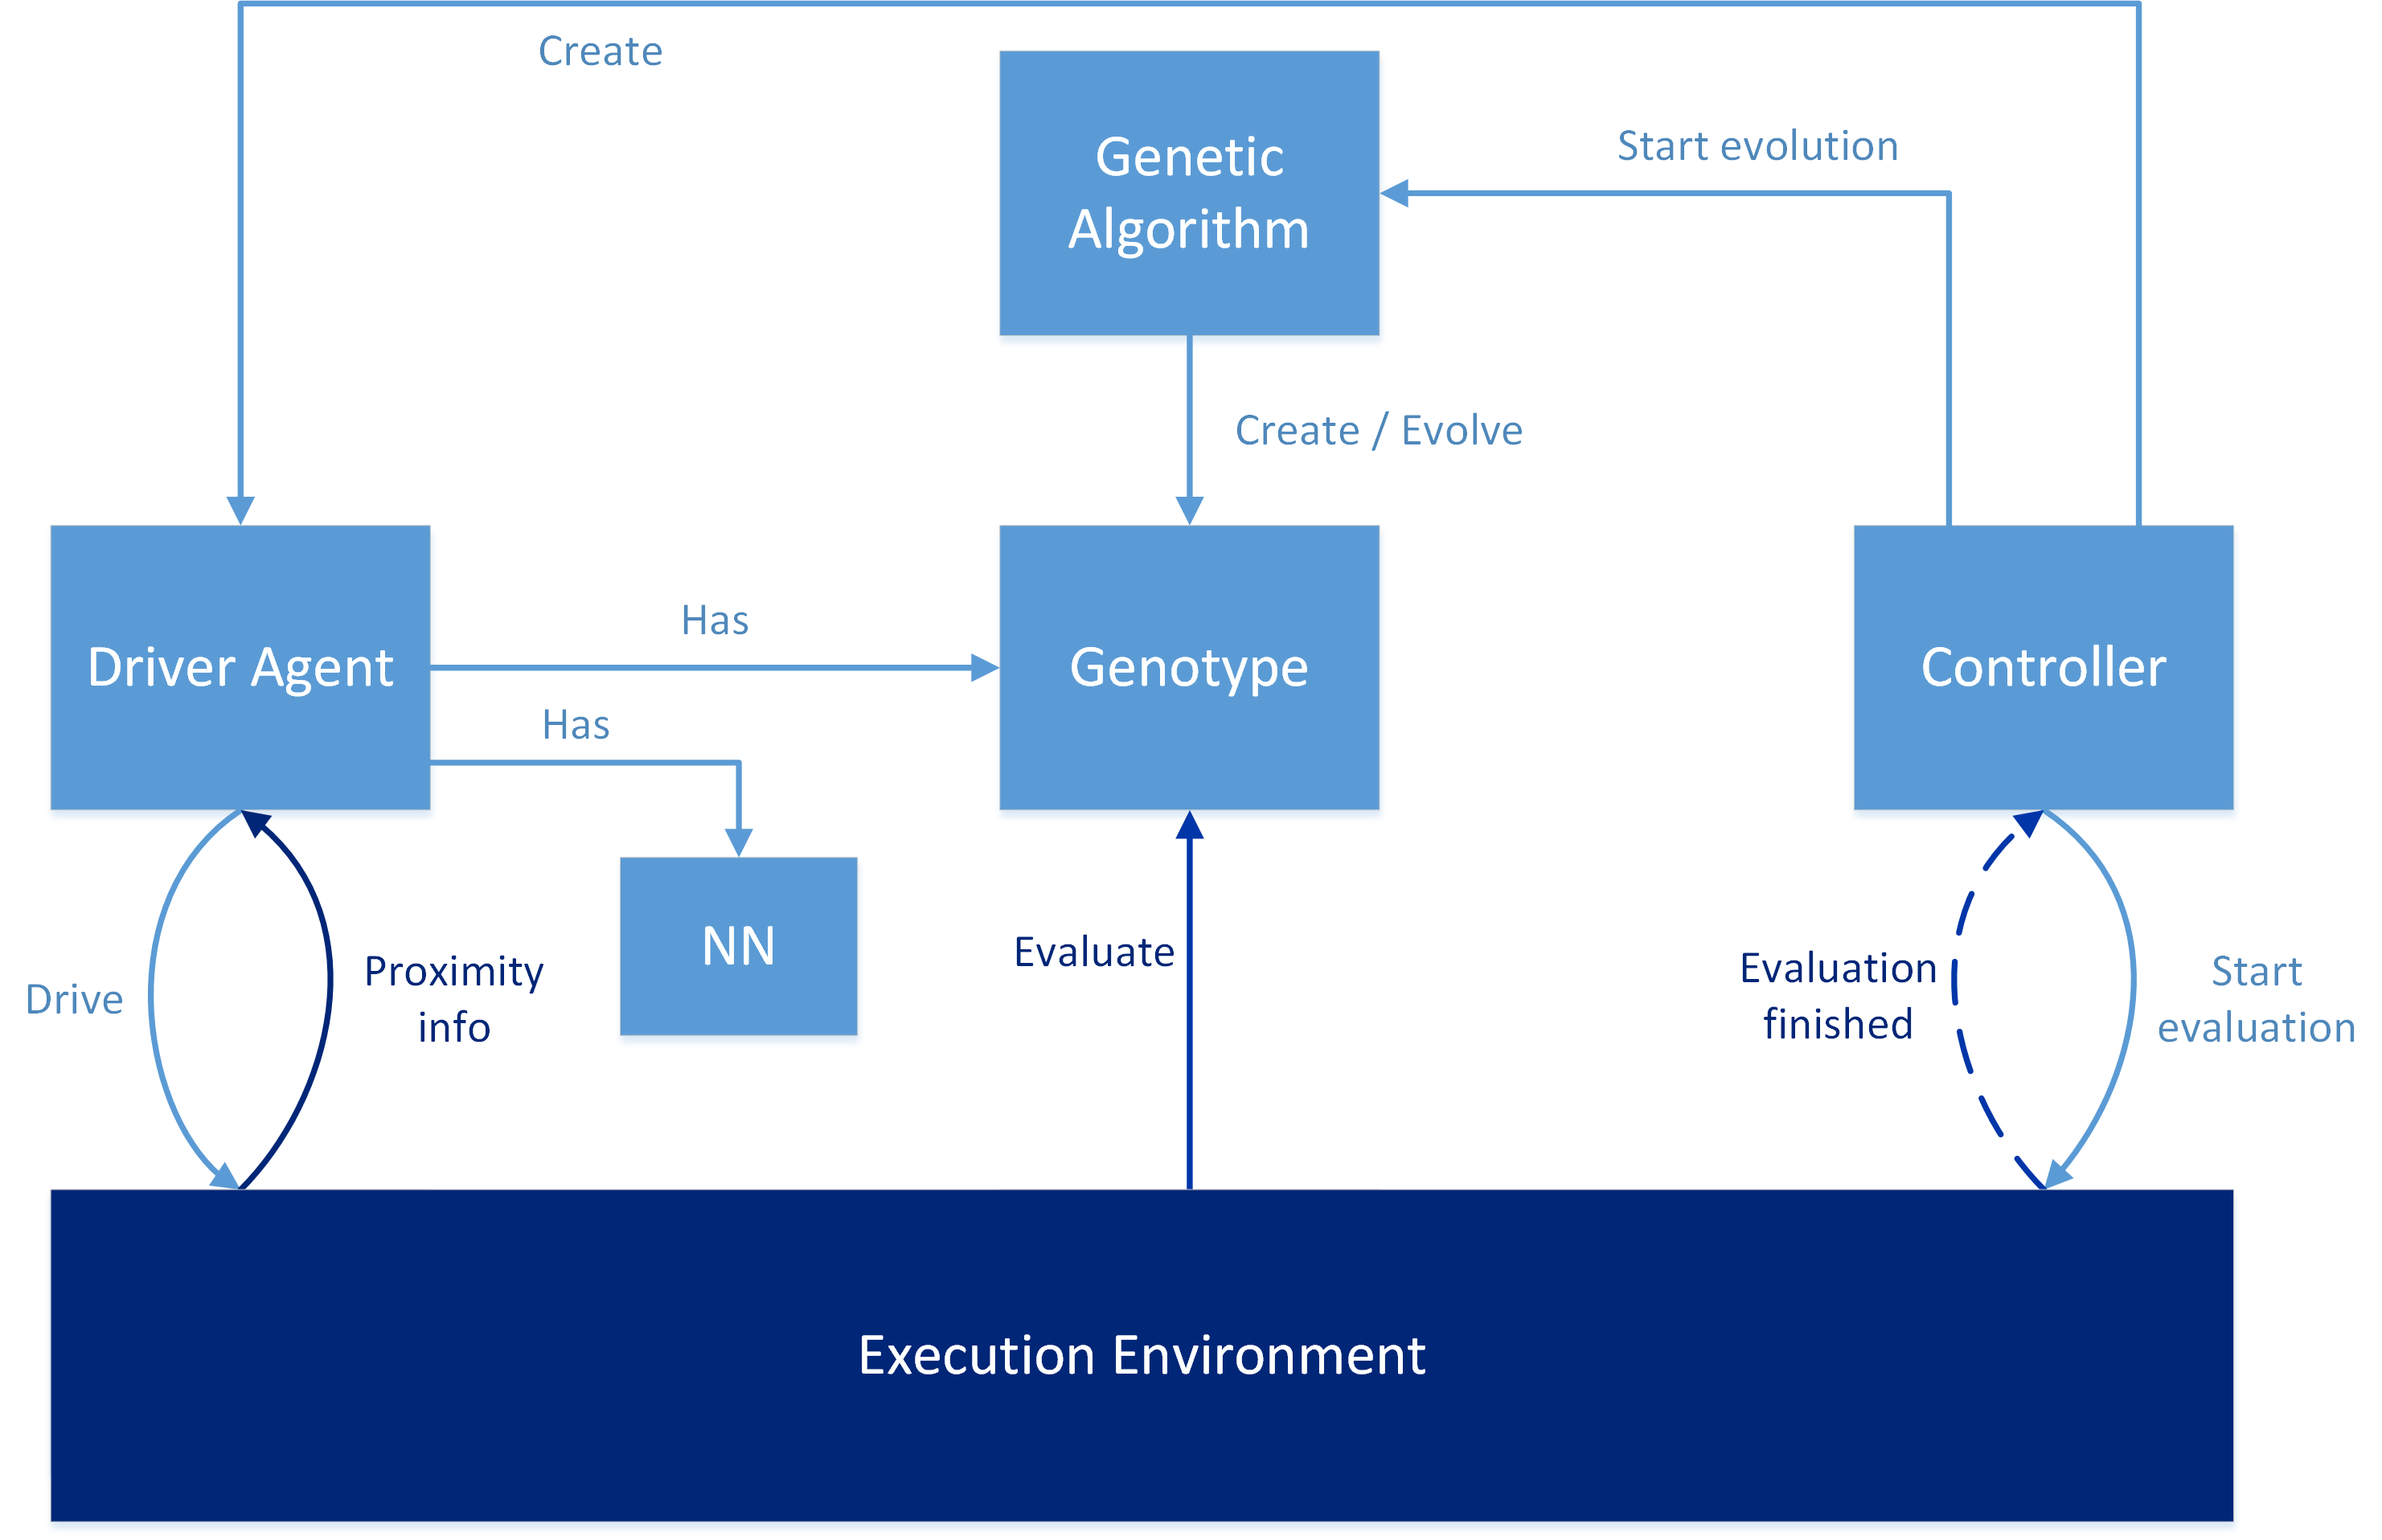
\includegraphics[width=130mm]{./img/architecture.png}
	\caption{Diagramma informale che rappresenta le relazioni tra i componenti che formano l'architettura del sistema. Nella notazione utilizzata, le frecce tratteggiate indicano una notifica dell'avvenimento di un certo evento, a differenza delle frecce continue che si riferiscono a relazioni di dipendenza. Nel diagramma sono rappresentati solamente i componenti relativi alla parte \emph{core} del sistema; quelli relativi all'ambiente di esecuzione non sono trattati in questo diagramma e sono, perciò, stati collassati nel blocco \emph{Execution Environment}.  \label{architecture-diagram}}
\end{figure}

\section{Evoluzione} \label{evolution}
In questa sezione verrà illustrata più nel dettaglio la parte inerente all'evoluzione del sistema, e al conseguente algoritmo genetico utilizzato. Molte scelte fatte si basano sul progetto \emph{Applying Evolutionary Artificial Neural Networks} \cite{arztRepo}, che è stato preso come punto di riferimento e come base per il nostro elaborato. Come accennato in precedenza la fase di evoluzione si divide in tre sottofasi distinte: \emph{selezione}, \emph{incrocio} (o \emph{crossover}) e \emph{mutazione}. Prima di procedere all'illustrazione di tali fasi, però, è necessario introdurre i parametri da noi utilizzati per valutare la bontà di un genotipo, e di conseguenza la sua fitness.
\subsection*{Evaluation e Fitness} \label{evFitness}
L'\emph{evaluation} rappresenta la bontà di un genotipo alla fine della fase di valutazione, ovvero, nel nostro caso, quanto bene l'auto è riuscita ad evitare i muri. Esso viene calcolato sulla base della distanza percorsa dall'auto, prendendo come origine il punto da cui essa parte all'inizio della fase di valutazione. Più un'auto farà strada prima di collidere contro un muro, maggiore sarà l'\emph{evaluation} del suo genoma. 

La fitness può essere calcolata in molti modi diversi, o addirittura fatta coincidere con l'\emph{evaluation}. L'approccio da noi scelto consiste nel calcolare la fitness come rapporto tra l'\emph{evaluation} di un individuo e l'\emph{evaluation} media della generazione. 
\begin{equation}
	fitness_i = \frac{evaluation_i}{\overline{ev}}, \hspace{2em} \overline{ev} = \frac{\sum_{j = 0}^{n} evaluation_j }{n}
\end{equation}
In questo modo la fitness di un individuo sarà maggiore di uno se la sua \emph{evaluation} è superiore alla media di tale generazione, ed inferiore nel caso contrario. Ciò è necessario per il metodo di selezione utilizzato, illustrato di seguito.
\subsection*{Selezione}
La fase di selezione, prendendo spunto da \cite{arztRepo}, avviene creando una generazione intermedia di potenziali ``\emph{genitori}'', che poi, riproducendosi tra loro, daranno vita ad una nuova generazione. Il metodo utilizzato per la creazione della generazione intermedia si basa sull'\emph{elitismo}, in modo che solamente gli individui migliori possano generare la nuova popolazione. In aggiunta a ciò, per mantenere una differenziazione genetica più elevata, vengono aggiunti alcuni genotipi di individui scelti in modo casuale.  

Come prima cosa vengono aggiunti alla generazione intermedia tutti i genotipi degli individui con fitness maggiore di uno (ovvero con \emph{evaluation} superiore alla media), in modo proporzionale al loro valore di fitness. Ciò significa che il genotipo di un individuo sarà inserito nella generazione intermedia tante volte quanto è il suo valore di fitness troncato all'intero. Ad esempio, se un individuo ha fitness 3.247, il suo genotipo sarà inserito nella generazione intermedia $\lfloor3.247\rfloor = 3$ volte. 

Dopo questa prima selezione per elitismo, ne viene fatta un'altra, in modo casuale. Come detto in precedenza ciò è utile per mantenere i genomi differenziati tra loro, e consente di esplorare strade che il solo elitismo non troverebbe. Il metodo utilizzato è il \emph{reminder stochastic sampling}, ed i genotipi da inserire nella generazione intermedia sono scelti nel seguente modo. Sia $r$ un numero casuale tra zero e uno, e $f = fitness_i - \lfloor fitness_i \rfloor$, ovvero la parte frazionaria della fitness. Se $r < f$ allora il genotipo viene inserito nella generazione intermedia.

Notare come la popolazione intermedia ottenuta dopo la fare di selezione non ha dimensione fissa. Essa ha l'unico vincolo di contenere almeno due genotipi, in modo che ci sia sempre una coppia per la successiva fase di riproduzione.
\subsection*{Crossover} \label{crossover}
Una volta ottenuta la popolazione intermedia di potenziali ``\emph{genitori}'' essi devono essere incrociati tra loro, per ottenere la nuova generazione. L'operatore di crossover da noi scelto è l'\emph{uniform crossover}, in cui ogni singolo gene è scelto dai due genitori in modo indipendente dagli altri. 

Per prima cosa vengono selezionati, in modo casuale, i due genitori dalla popolazione intermedia. Ogni coppia così selezionata produce due figli nel modo seguente: 
\begin{enumerate}
	\item Siano parent\textsubscript{1} e parent\textsubscript{2} i due genitori e offspring\textsubscript{1} e offspring\textsubscript{2} i due discendenti.
	\item Sia $p_{cross}$, tra zero ed uno, la probabilità di crossover.
	\item Per ogni gene all'interno dei genotipi si estrae un numero casuale $r$, tra zero ed uno. Se $r < p_{cross}$ allora avviene il crossover, e offspring\textsubscript{1} eredita il gene da parent\textsubscript{2}, mentre offspring\textsubscript{2} lo eredita da parent\textsubscript{1}. In caso contrario offspring\textsubscript{1} eredita il gene da parent\textsubscript{1}, e offspring\textsubscript{2} lo eredita da parent\textsubscript{2}.
	\item Una volta fatto ciò per ogni gene nel genotipo, si inseriscono i due nuovi genomi nella nuova generazione, uno per volta, fino a raggiungere la dimensione desiderata. 
\end{enumerate}
Durante prove sperimentali abbiamo notato come, spesso, un genoma molto buono vada perso nella generazione successiva, vanificando di conseguenza i progressi fatti fino a quel momento. Per risolvere tale problematica abbiamo leggermente modificato il metodo proposto in precedenza, inserendo nella nuova generazione i genotipi degli $m$ individui con la migliore fitness della generazione precedente.
\subsection*{Mutazione} \label{mutazione}
Dopo la composizione della nuova generazione i genotipi dei nuovi individui vengono mutati. La mutazione, all'interno di un genotipo, viene eseguita gene per gene, su basi probabilistiche. Di seguito è riportato lo pseudo-codice dell'algoritmo di mutazione:
\begin{enumerate}
	\item Sia $p_{gt}$ la probabilità, tra zero e uno, che un genotipo sia selezionato per la mutazione dei sui geni. Sia $p_{gn}$ la probabilità, tra zero e uno, che un gene sia mutato. Infine sia $mut_{max}$ il massimo livello di mutazione di un gene (un gene può essere mutato di massimo $\pm mut_{max}$).
	\item Per ogni genotipo nella nuova generazione viene estratto un numero random $r_1$ tra zero ed uno. Se $r_1 < p_{gt}$ allora il genotipo è selezionato per la mutazione, altrimenti non viene mutato.
	\item Per ogni gene dei genotipi selezionati al passo 2. viene estratto un numero casuale $r_2$ tra zero ed uno. Se $r_2 < p_{gn}$ il gene viene mutato, di una quantità pari a $r_3 \cdot (mut_{max} \cdot 2) - mut_{max}$, dove $r_3$ è un numero casuale tra zero ed uno. Tale quantità viene aggiunta al valore del gene. Nel nostro caso non c'è un limite al valore che i geni possono assumere. 
\end{enumerate}
In \autoref{crossover}, per fare in modo di non perdere i progressi fatti dalle generazioni precedenti, i genotipi degli $m$ individui migliori venivano direttamente passati nella generazione successiva. Essi non devono quindi venire mutati. Per tale motivo l'algoritmo per la mutazione proposto in precedenza non viene eseguito per i primi $m$ genotipi nella nuova generazione, che non saranno perciò mutati.
\subsection*{Valori dei parametri} \label{valore-dei-parametri}
In questa sezione verranno esplicitati i valori dei parametri dell'algoritmo genetico precedentemente illustrato. Tali parametri sono stati utilizzati per le prove sperimentali, descritte in \autoref{risultati}. Il valore di tali parametri non è stato sperimentalmente ricavato tramite \emph{fine tuning}, e perciò non necessariamente rappresentano i migliori valori possibili. La maggior parte di tali valori sono stati ricavati da quelli utilizzati in \cite{arztRepo}, o tramite alcuni semplici test sperimentali.

\begin{center}
	\begin{tabular}{| m{2.5cm} | m{6cm} | m{2cm} |}
		\hline
		\textbf{Parametro} & \textbf{Commento}& \textbf{Valore} \\ \hline
		$p_{cross}$ & Probabilità di crossover tra i geni di due genitori (vedi \autoref{crossover})  & $0.6$ \\ \hline
		$p_{gt}$ & Probabilità che un genotipo sia selezionato per la mutazione* (vedi \autoref{mutazione})  & $1.0$ \\ \hline
		$p_{gn}$ & Probabilità che un singolo gene sia mutato (vedi \autoref{mutazione})  & $0.3$ \\ \hline
		$mut_{max}$ & Massimo valore di cui può essere mutato un gene (vedi \autoref{mutazione})  & $\pm 2$ \\ \hline
		$m$ & Numero dei genotipi migliori che vengono passati direttamente nella generazione successiva (vedi \autoref{crossover})  & $1$ \\ \hline
	\end{tabular}
	\begin{tablenotes}
		*Gli $m$ genotipi migliori della generazione precedente non vengono mai mutati.
	\end{tablenotes}
\end{center} 

\section{Simulazione} \label{simulation}
% bisogna spiegare perchè l'evaluation è fatta da un componente della simulazione e non da uno del core
% oltre all'evaluation, bisogna spiegare anche il timeout
L'architettura illustrata in \autoref{architecture} mette in evidenza i componenti principali del sistema. Come anticipato, per completare l'architettura si rivela necessaria l'aggiunta di ulteriori componenti, dipendenti dall'ambiente di esecuzione. Nel progetto in esame, si è scelto di simulare l'ambiente di esecuzione attraverso l'utilizzo di un motore grafico. Il blocco \emph{Execution Environment}, presente in \autoref{architecture-diagram}, è stato raffinato nei seguenti componenti.
\begin{description}
	\item[Car]: rappresenta un'auto. È equipaggiata con cinque sensori di prossimità in grado di percepire la distanza da eventuali ostacoli o muri. Più nello specifico, ogni sensore è posizionato secondo una certa angolazione rispetto all'asse dell'auto, da \ang{-60} fino a \ang{+60}. In questo modo è possibile effettuare una completa operazione di \emph{sensing} nella zona frontale rispetto al veicolo. Ogni auto è associata ad un \emph{Driver Agent}, al quale deve inoltrare i valori rilevati dai sensori per ottenere indicazioni sullo spostamento da effettuare. Se dai sensori viene rilevata una collisione con i muri del tracciato, l'auto si ferma immediatamente, notificando il \emph{Race Manager}.
	\item[Race Manager]: è il componente dedito all'esecuzione della fase di \emph{evaluation} di ogni generazione dell'algoritmo genetico. Più nel dettaglio, all'avvio ha il compito di creare auto e tracciato, mentre durante l'evaluation è responsabile del controllo dello stato di ogni auto. All'inizio di ogni iterazione, si occupa del riposizionamento di ogni auto all'inizio del tracciato. Al termine dell'iterazione, ovvero quando tutte le auto hanno segnalato una collisione o hanno terminato il tracciato, provvede ad assegnare una valutazione al genotipo corrispondente ad ogni auto e a notificare il \emph{Controller}.
	\item[Track]: rappresenta il tracciato, circondato da muri, sul quale si muovono le auto. Su di esso sono disposti dei \emph{checkpoint}, utilizzabili per effettuare l'evaluation del genotipo di ogni auto. I checkpoint sono posizionati, in maniera uniforme, per tutta la lunghezza del tracciato. Il raggiungimento dell'ultimo di essi sancisce il completamento del tracciato.
\end{description}
I componenti appena descritti sono rappresentati in \autoref{simulation-diagram}, insieme all'architettura generale del sistema. Per quanto riguarda la fase di valutazione dei genotipi, si sono adottate come riferimento le indicazioni presenti in \autoref{evolution}. Siccome nel calcolo dell'\emph{evaluation} l'unica dimensione presa in considerazione è la distanza percorsa dalle auto, si è rivelato necessario aggiungere anche un vincolo temporale ad ogni iterazione. Seguendo questo approccio, è stato assegnato un timeout ad ogni auto, ovvero un tempo massimo per raggiungere il checkpoint successivo. Il timeout viene resettato al raggiungimento di ogni checkpoint e una sua scadenza significa che l'auto in questione non sta effettuando alcun progresso nel tracciato e quindi deve essere fermata. In questo modo, si evita che le auto rimangano in corsa pur stando ferme in un punto, forzandole a progredire nel tracciato. Il controllo relativo ai timeout è gestito dal componente \emph{Race Manager}.

\begin{figure}[H]
	\centering
	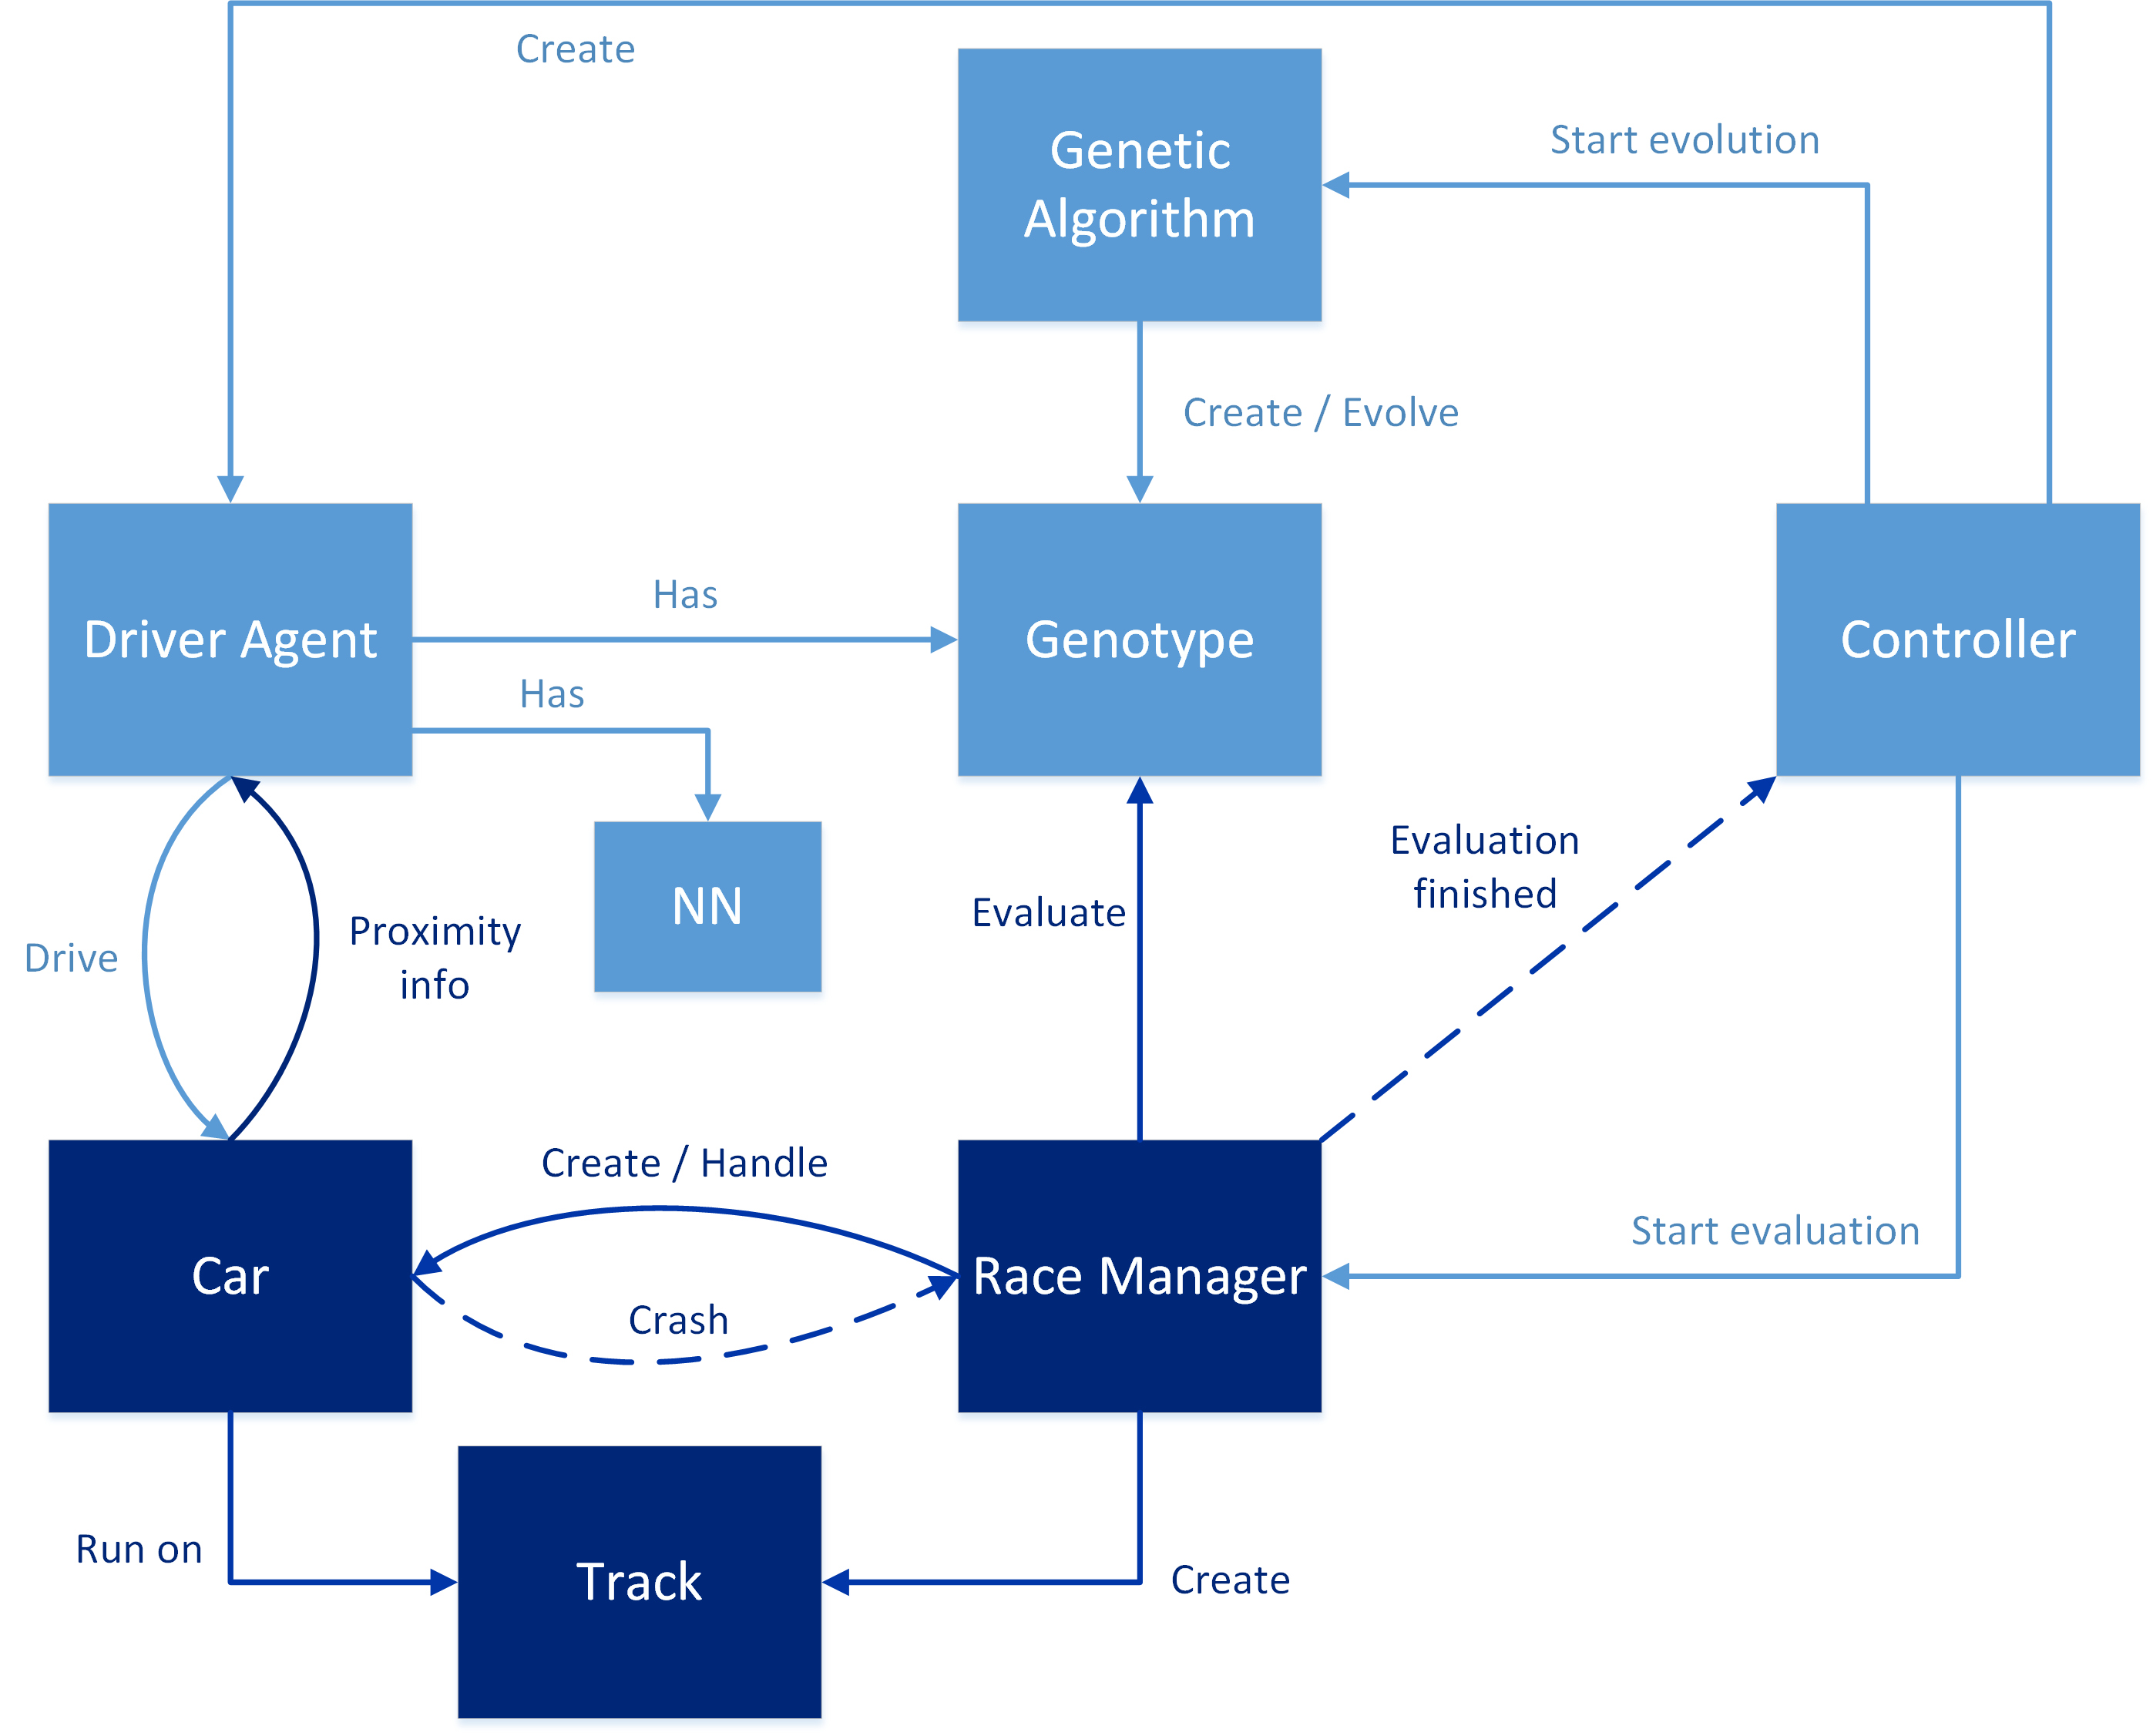
\includegraphics[width=130mm]{./img/architecture-simulation.png}
	\caption{Diagramma informale che rappresenta le relazioni tra i componenti che formano l'architettura del sistema. Nella notazione utilizzata, le frecce tratteggiate indicano una notifica dell'avvenimento di un certo evento, a differenza delle frecce continue che si riferiscono a relazioni di dipendenza. Nel diagramma i componenti caratterizzati da un colore più scuro sono quelli relativi alla simulazione, distinguibili dai restanti che costituiscono invece il \emph{core} del sistema.  \label{simulation-diagram}}
\end{figure}

In questa sezione è stata proposta una possibile architettura per la parte del sistema relativa all'ambiente di esecuzione. L'implementazione dei componenti relativi alla parte dell'ambiente di esecuzione non può essere sviluppata in maniera generale, ma contiene, necessariamente, dei riferimenti all'ambiente stesso. In questo progetto l'ambiente di esecuzione è stato simulato tramite l'utilizzo del motore grafico \emph{Godot}\footnote{\url{https://godotengine.org/}}. Nel caso si voglia adottare un differente ambiente di esecuzione, sia reale che simulato, sarà sufficiente variare l'implementazione dei componenti \emph{Car}, \emph{Race Manager} e \emph{Track} in modo da adattarli all'ambiente scelto. Non sarà necessario apportare modifiche al \emph{core}, a patto che vengano preservate le interazioni tra le due parti del sistema, descritte nell'architettura in \autoref{architecture}.

\section{Risultati} \label{risultati}
In questa sezione verranno analizzati i risultati ottenuti tramite prove sperimentali del sistema. Per gli esperimenti sono stati utilizzati quattro diversi tracciati, con diversi gradi di difficoltà (codificati in \emph{facile}, \emph{medio-facile}, \emph{medio-difficile}, \emph{difficile}). I tracciati sono visibili in \autoref{fig:tracks}. Alcuni esempi di esecuzioni del sistema sono disponibili in \cite{ourRepo}.
\begin{figure}[H]
	\centering
	\begin{subfigure}[b]{0.475\textwidth}
		\centering
		
\includegraphics[width=\textwidth]{./img/track01.png}
		\caption[Network2]%
		{{\small Circuito 1 - medio-facile}}    
	\end{subfigure}
	\hfill
	\begin{subfigure}[b]{0.475\textwidth}  
		\centering 
		
\includegraphics[width=\textwidth]{./img/track02.png}
		\caption[]%
		{{\small Circuito 2 - facile}}
	\end{subfigure}
	\vskip\baselineskip
	\begin{subfigure}[b]{0.475\textwidth}   
		\centering 
		
\includegraphics[width=\textwidth]{./img/track03.png}
		\caption[]%
		{{\small Circuito 3 - medio-difficile}}
	\end{subfigure}
	\quad
	\begin{subfigure}[b]{0.475\textwidth}   
		\centering 
		
\includegraphics[width=\textwidth]{./img/track04.png}
		\caption[]%
		{{\small Circuito 4 - difficile}}
	\end{subfigure}
	\caption[]
	{\small I tracciati utilizzati nelle simulazioni. Viene visualizzato anche il punto di partenza delle auto.} 
	\label{fig:tracks}
\end{figure}
La durata degli esperimenti è stata impostata a 50 generazioni, in modo che, per ogni tracciato, almeno un'auto raggiunga la fine dello stesso, identificata dall'ultimo checkpoint. Tale valore è stato settato dopo varie prove, ed ha il solo scopo di soddisfare il requisito sopra espresso. Per ogni tracciato sono stati eseguiti cinque test differenti (un singolo test può durare più di 20 minuti, e ci si è limitati a cinque per tracciato per motivi di tempo). In ogni test è stata tenuta traccia dell'\emph{evaluation} media e massima ad ogni generazione. Non è stata utilizzata la fitness poiché, per come è stata calcolata in questo progetto (vedi \autoref{evFitness}), essa esprime solamente di quanto una singola auto è stata migliore (o peggiore) della media della propria generazione, e quindi essa non rappresenta un dato significativo per tutta la generazione. 

I tracciati hanno lunghezze diverse, e quindi le corrispettive \emph{evaluation} sono differenti. Per tale motivo, quando essi vengono confrontati, non si fa riferimento all'\emph{evaluation}, ma alla percentuale di completamento. I grafici dei dati raccolti durante gli esperimenti sono consultabili di seguito.

\begin{figure}[H]
	\centering
	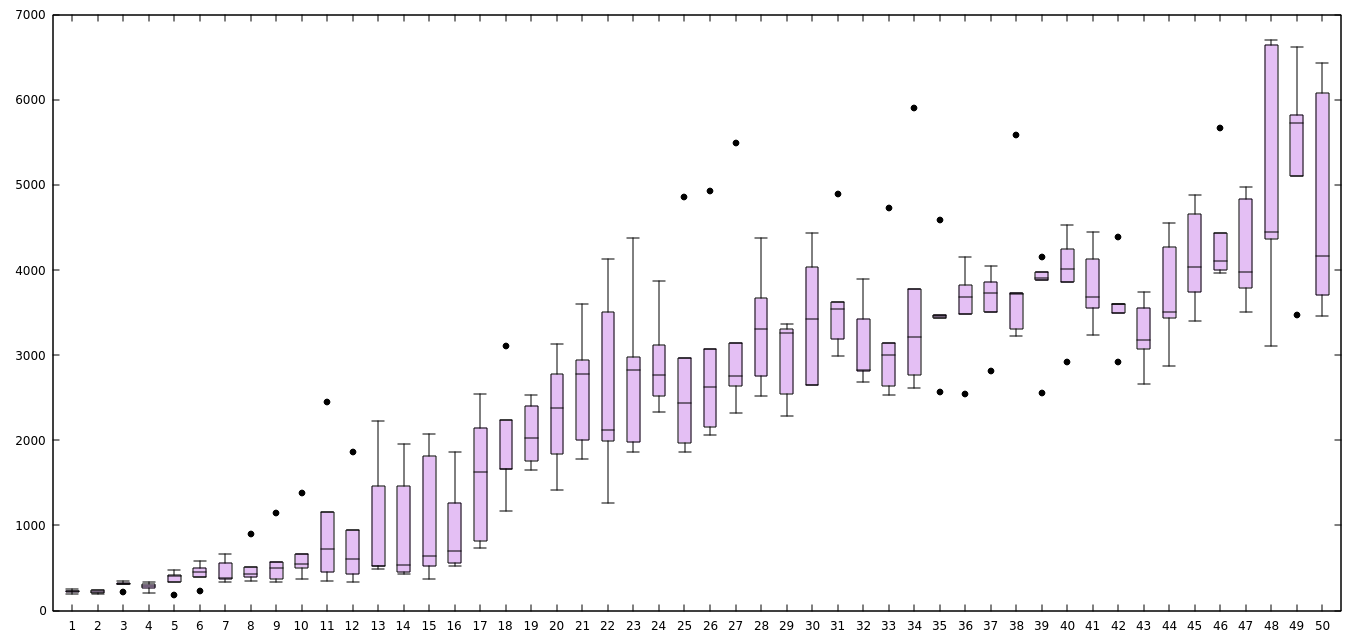
\includegraphics[width=130mm]{../results/track01/averageEvaluation.png}
	\caption{Grafico che mostra l'andamento dell'\emph{evaluation} media durante le 50 generazioni nel tracciato 1 (medio-facile). Tale grafico raggruppa i valori di cinque esperimenti, e per tale motivo i dati sono visualizzati tramite \emph{boxplot}. Si può notare che l'\emph{evaluation} media ha un andamento per lo più crescente al crescere del numero di generazioni, indicando che le auto, mediamente, fanno più strada prima di collidere con i muri del tracciato, al crescere della generazione.}
\end{figure}

\begin{figure}[H]
	\centering
	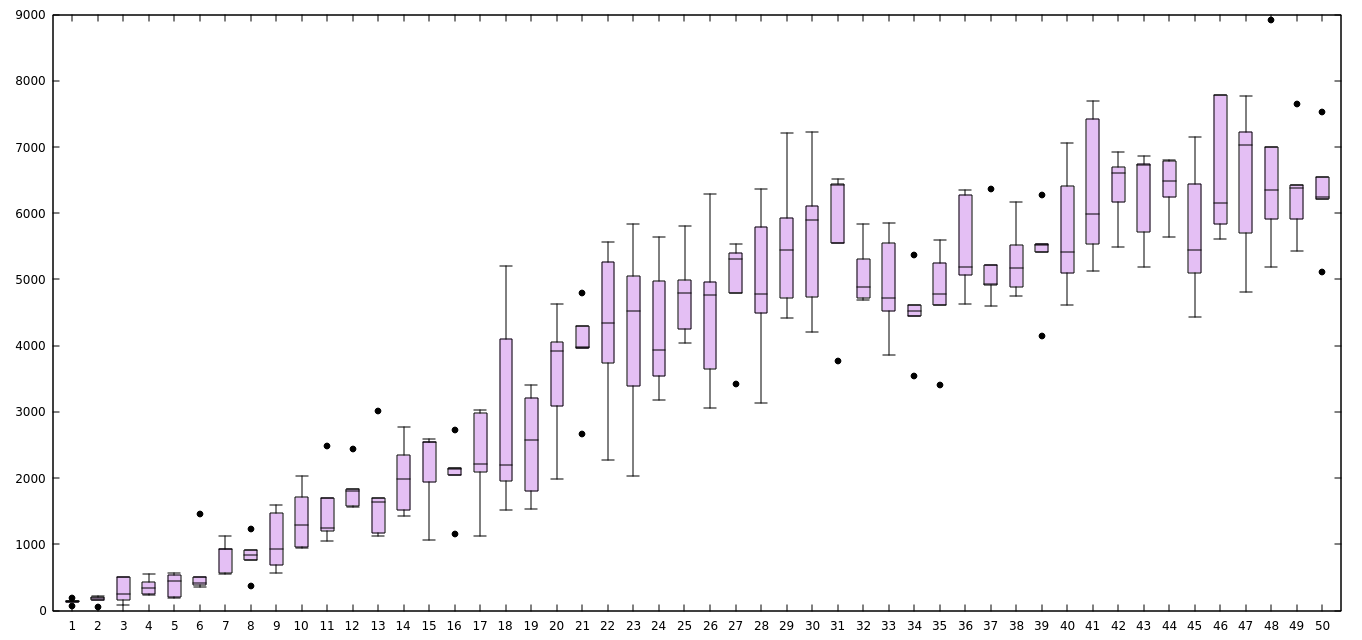
\includegraphics[width=130mm]{../results/track02/averageEvaluation.png}
	\caption{Grafico che mostra l'andamento dell'\emph{evaluation} media durante le 50 generazioni nel tracciato 2 (facile). Come per i grafici precedenti esso raggruppa, tramite \emph{boxplot}, i valori di cinque diversi esperimenti. Anche in questo caso l'andamento dell'\emph{evaluation} media è crescente al crescere delle generazioni, certificando la bontà delle soluzioni adottate. }
\end{figure}

\begin{figure}[H]
	\centering
	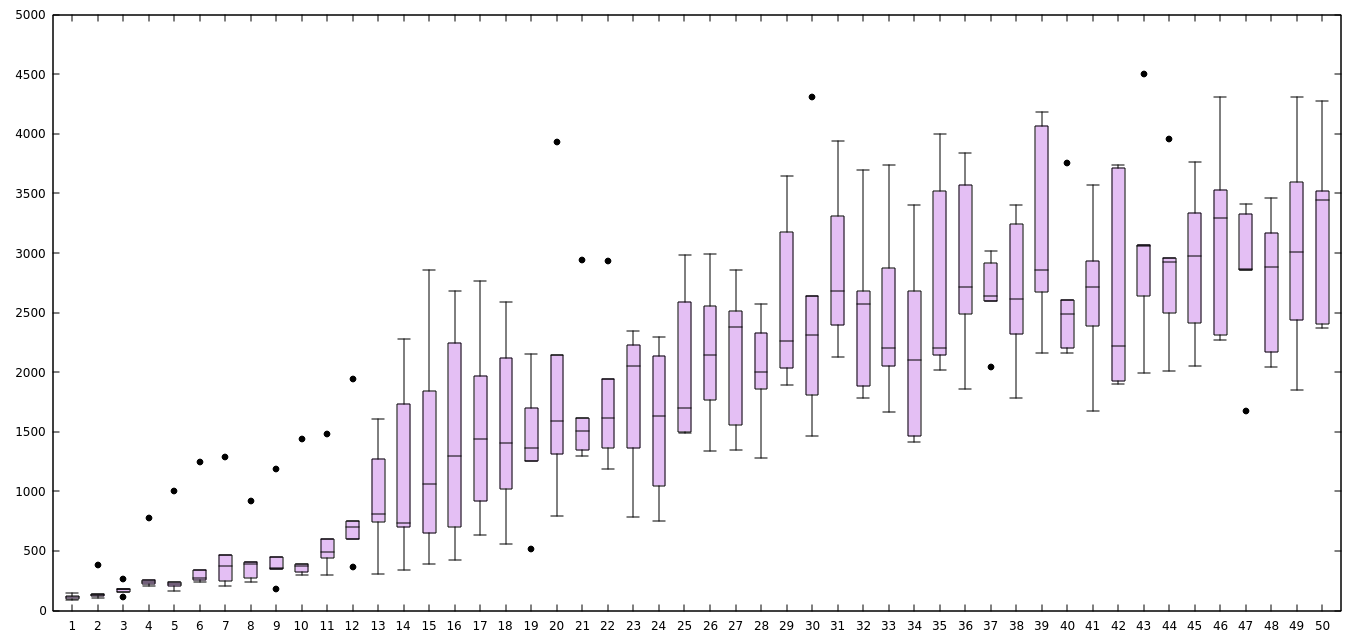
\includegraphics[width=130mm]{../results/track03/averageEvaluation.png}
	\caption{Grafico che mostra l'andamento dell'\emph{evaluation} media durante le 50 generazioni nel tracciato 3 (medio-difficile). Come per i grafici precedenti esso raggruppa, tramite \emph{boxplot}, i valori di cinque diversi esperimenti. Anche in questo caso l'andamento dell'\emph{evaluation} media è crescente al crescere delle generazioni, certificando la bontà delle soluzioni adottate. }
\end{figure}

\begin{figure}
	\centering
	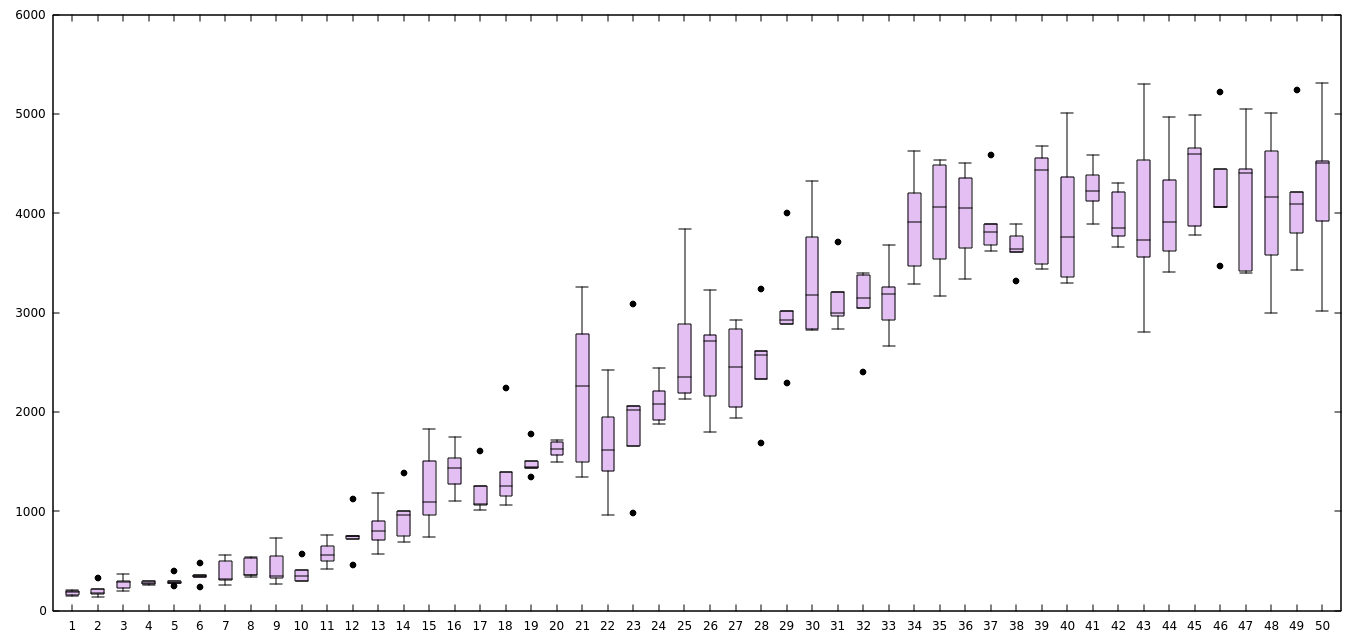
\includegraphics[width=130mm]{../results/track04/averageEvaluation.png}
	\caption{Grafico che mostra l'andamento dell'\emph{evaluation} media durante le 50 generazioni nel tracciato 4 (difficile). Come per i grafici precedenti esso raggruppa, tramite \emph{boxplot}, i valori di cinque diversi esperimenti. Anche in questo caso l'andamento dell'\emph{evaluation} media è crescente al crescere delle generazioni, certificando la bontà delle soluzioni adottate. }
\end{figure}

\begin{figure}[H]
	\centering
	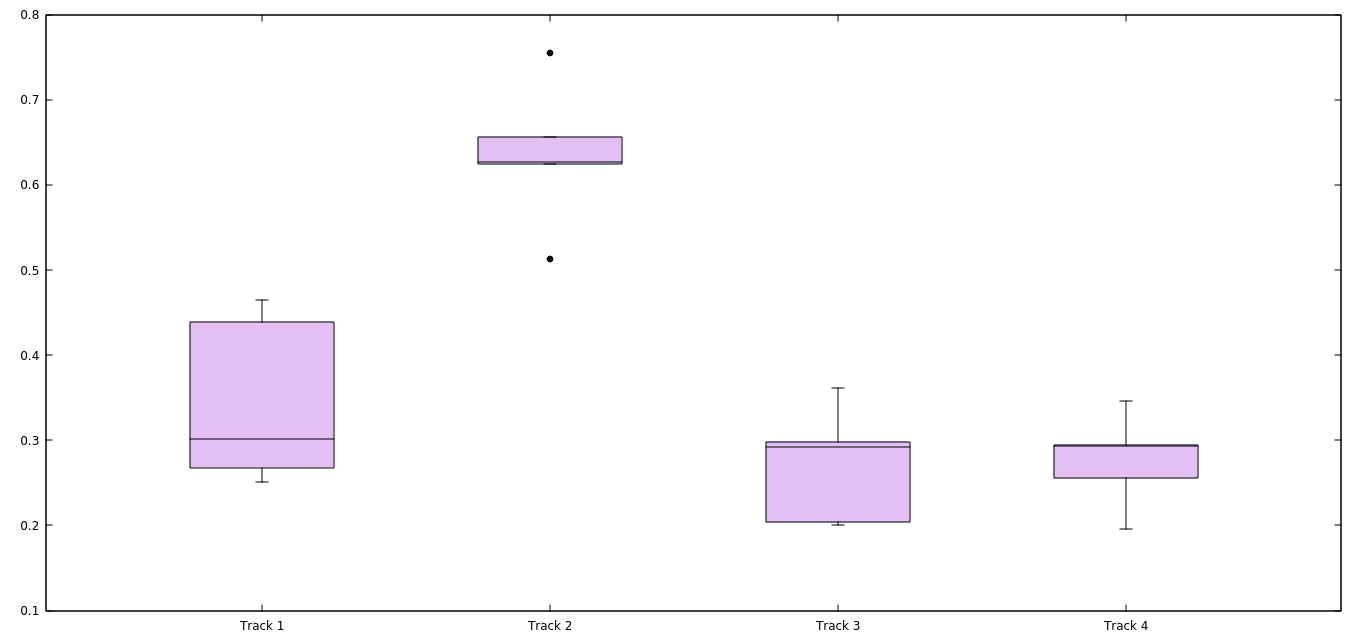
\includegraphics[width=130mm]{../results/avgEvAtTheEnd.png}
	\caption{Confronto dei valori di \emph{evaluation} media per i quattro tracciati alla fine dei test (alla 50esima generazione). Come accennato in precedenza, i tracciati hanno lunghezze diverse, e dato che l'\emph{evaluation} è direttamente proporzionale alla distanza percorsa, essi non sono direttamente confrontabili. Per ovviare a questo problema è stata usata la percentuale di completamento del tracciato, ovvero al posto di considerare l'\emph{evaluation} si considera il completamento, dato da \emph{evaluation} dell'auto diviso l'\emph{evaluation} massima per un dato circuito. Quello qui rappresentato è, quindi, il livello medio di completamento del tracciato, alla 50esima generazione. Come si può notare, il tracciato 2 (il più semplice) ha una percentuale media di completamento più alta, mentre gli altri tracciati presentano dati simili. Il tracciato 3 presenta una media di completamento molto bassa, a causa della particolare conformazione ``a strettoia'', che non consente a molte auto di superare le prime asperità. Come per gli altri grafici sono raggruppati i risultati di cinque simulazioni, tramite \emph{boxplot}.}
\end{figure}


\section{Conclusioni} \label{conclusions}

Siamo complessivamente soddisfatti del lavoro svolto: grazie all'algoritmo genetico sviluppato, le auto riescono a completare tutti e quatto i circuiti da noi creati. Più nel dettaglio, i più difficili vengono completati, in media, attorno alla trentesima generazione.

I risultati mostrano che il processo evolutivo da noi sviluppato è efficace e la popolazione di auto mostra un miglioramento tendenzialmente costante al crescere del numero di generazioni. Inoltre non è presente \emph{overfitting} dell'algoritmo per una particolare tipologia di tracciato, dato che i tracciati da noi utilizzati sono piuttosto differenti l'uno dall'altro, e per ognuno di essi sono stati ottenuti buoni risultati. In più i gradi di difficoltà stimati inizialmente per ogni tracciato si sono rivelati corretti anche a fronte dei test sperimentali. 

\subsection*{Sviluppi futuri}

Per quanto concerne gli sviluppi futuri, si individuano due modalità principali per estendere il sistema realizzato: modifiche all'algoritmo genetico o aggiunta di nuove funzionalità.

\subsubsection*{Algoritmo genetico} 

\begin{itemize}
	\item \textbf{Tuning dei parametri} : nonostante l'algoritmo genetico realizzato abbia conferito buoni risultati, si potrebbe indagare sulla bontà dei parametri che esso utilizza, elencati in \autoref{valore-dei-parametri}. Siccome l'algoritmo si basa su nozioni probabilistiche, tali parametri svolgono un ruolo fondamentale nella fase di evoluzione. A causa di vincoli temporali non è stato possibile, però, tarare questi parametri nel modo più accurato.
	\item \textbf{Nuovi operatori di selezione, crossover e mutazione} : le fasi di selezione, crossover e mutazione possono essere svolte in svariati modi, illustrati in parte in \autoref{stato-dell-arte}. Anche in questo caso, a causa di vincoli temporali, sono stati scelti i tre operatori in base alle motivazioni illustrate in \autoref{evolution}. Sarebbe quindi opportuno testare la bontà di strategie differenti per la fase di evoluzione.
\end{itemize}
 

\subsubsection*{Nuove funzionalità}

\begin{itemize}
	\item \textbf{Realizzazione di una gara} : allo stato attuale, l'obiettivo delle auto è quello di completare il tracciato senza dare importanza al tempo impiegato. Nel caso si volesse realizzare una gara tra auto, sarebbe necessario modificare la strategia utilizzata per il calcolo dell'evaluation, tenendo conto anche della velocità media delle auto in modo da premiare quelle più veloci.
	\item \textbf{Livello di energia} : si può pensare di assegnare un certo livello di energia ad ogni auto, non sufficiente per completare il tracciato. Ogni auto avrà la possibilità, in qualunque momento, di procedere alla ricarica (possibile una sola volta). Durante la ricarica essa rimarrà ferma per un dato periodo di tempo. Quindi, oltre a determinare velocità e direzione del prossimo spostamento, ogni auto dovrà valutare il momento più opportuno per eseguire la ricarica.
	\item \textbf{Utilizzo di più tipologie di veicoli} : allo stato attuale, è possibile far correre sul tracciato solo un tipo predefinito di auto, avente una certa dimensione e caratterizzata da una propria velocità massima e da un proprio angolo massimo di sterzatura. Sarebbe interessante progettare ed aggiungere nuove tipologie di veicoli, aventi dimensione, velocità massima e sterzatura massima differenti. In aggiunta, ogni tipologia potrebbe essere evoluta in modo completamente indipendente dalle altre. 
\end{itemize}

\newpage
\begin{thebibliography}{1}
	\bibitem{arztRepo}{Samuel Arzt, \emph{Applying Evolutionary Artificial Neural Networks} \\ URL:  \url{https://github.com/ArztSamuel/Applying_EANNs}\\ Ultima visita: 8 Luglio 2018}
	
	\bibitem{ourRepo}{Gabriele Graffieti, Alfredo Maffi, Manuel Peruzzi \emph{evolutionary-cars} \\ URL:  \url{https://github.com/manuelperuzzi/evolutionary-cars}\\ Ultima visita: 9 Luglio 2018}
	
	\bibitem{ref_paper} António Carlos Gomes Rodrigues Marques Simões, {\em Automatic vehicle classification using appearance based features}, 2015.
	
\end{thebibliography}

\end{document}
